%%%%%%%%%%%%%%%%%%%%%%%%%%%%%%%%%%%%%%%%%
% Structured General Purpose Assignment
% LaTeX Template
%
% This template has been downloaded from:
% http://www.latextemplates.com
%
% Original author:
% Ted Pavlic (http://www.tedpavlic.com)
%
% Note:
% The \lipsum[#] commands throughout this template generate dummy text
% to fill the template out. These commands should all be removed when 
% writing assignment content.
%
%%%%%%%%%%%%%%%%%%%%%%%%%%%%%%%%%%%%%%%%%

%----------------------------------------------------------------------------------------
%	PACKAGES AND OTHER DOCUMENT CONFIGURATIONS
%----------------------------------------------------------------------------------------

\documentclass{article}

\usepackage{fancyhdr} % Required for custom headers
\usepackage{lastpage} % Required to determine the last page for the footer
\usepackage{extramarks} % Required for headers and footers
\usepackage{graphicx} % Required to insert images
\usepackage{lipsum} % Used for inserting dummy 'Lorem ipsum' text into the template
\usepackage{listings}
\usepackage{color}
\usepackage{amsmath}

\definecolor{dkgreen}{rgb}{0,0.6,0}
\definecolor{gray}{rgb}{0.5,0.5,0.5}
\definecolor{mauve}{rgb}{0.58,0,0.82}

\lstset{frame=tb,
  language=python,
  aboveskip=3mm,
  belowskip=3mm,
  showstringspaces=false,
  columns=flexible,
  basicstyle={\small\ttfamily},
  numbers=none,
  numberstyle=\tiny\color{gray},
  keywordstyle=\color{blue},
  commentstyle=\color{dkgreen},
  stringstyle=\color{mauve},
  breaklines=true,
  breakatwhitespace=true
  tabsize=3
}

% Margins
\topmargin=-0.45in
\evensidemargin=0in
\oddsidemargin=0in
\textwidth=6.5in
\textheight=9.0in
\headsep=0.25in 

\linespread{1.1} % Line spacing

% Set up the header and footer
\pagestyle{fancy}
\lhead{\hmwkAuthorName} % Top left header
\chead{\hmwkClass\ (\hmwkClassInstructor\ \hmwkClassTime): \hmwkTitle} % Top center header
\rhead{\firstxmark} % Top right header
\lfoot{\lastxmark} % Bottom left footer
\cfoot{} % Bottom center footer
\rfoot{Page\ \thepage\ of\ \pageref{LastPage}} % Bottom right footer
\renewcommand\headrulewidth{0.4pt} % Size of the header rule
\renewcommand\footrulewidth{0.4pt} % Size of the footer rule

\setlength\parindent{0pt} % Removes all indentation from paragraphs

%----------------------------------------------------------------------------------------
%	DOCUMENT STRUCTURE COMMANDS
%	Skip this unless you know what you're doing
%----------------------------------------------------------------------------------------

% Header and footer for when a page split occurs within a problem environment
\newcommand{\enterProblemHeader}[1]{
\nobreak\extramarks{#1}{#1 continued on next page\ldots}\nobreak
\nobreak\extramarks{#1 (continued)}{#1 continued on next page\ldots}\nobreak
}

% Header and footer for when a page split occurs between problem environments
\newcommand{\exitProblemHeader}[1]{
\nobreak\extramarks{#1 (continued)}{#1 continued on next page\ldots}\nobreak
\nobreak\extramarks{#1}{}\nobreak
}

\setcounter{secnumdepth}{0} % Removes default section numbers
\newcounter{homeworkProblemCounter} % Creates a counter to keep track of the number of problems

\newcommand{\homeworkProblemName}{}
\newenvironment{homeworkProblem}[1][Problem \arabic{homeworkProblemCounter}]{ % Makes a new environment called homeworkProblem which takes 1 argument (custom name) but the default is "Problem #"
\stepcounter{homeworkProblemCounter} % Increase counter for number of problems
\renewcommand{\homeworkProblemName}{#1} % Assign \homeworkProblemName the name of the problem
\section{\homeworkProblemName} % Make a section in the document with the custom problem count
\enterProblemHeader{\homeworkProblemName} % Header and footer within the environment
}{
\exitProblemHeader{\homeworkProblemName} % Header and footer after the environment
}

\newcommand{\problemAnswer}[1]{ % Defines the problem answer command with the content as the only argument
\noindent\framebox[\columnwidth][c]{\begin{minipage}{0.98\columnwidth}#1\end{minipage}} % Makes the box around the problem answer and puts the content inside
}

\newcommand{\homeworkSectionName}{}
\newenvironment{homeworkSection}[1]{ % New environment for sections within homework problems, takes 1 argument - the name of the section
\renewcommand{\homeworkSectionName}{#1} % Assign \homeworkSectionName to the name of the section from the environment argument
\subsection{\homeworkSectionName} % Make a subsection with the custom name of the subsection
\enterProblemHeader{\homeworkProblemName\ [\homeworkSectionName]} % Header and footer within the environment
}{
\enterProblemHeader{\homeworkProblemName} % Header and footer after the environment
}
   
%----------------------------------------------------------------------------------------
%	NAME AND CLASS SECTION
%----------------------------------------------------------------------------------------

\newcommand{\hmwkTitle}{Assignment\ \#4} % Assignment title
\newcommand{\hmwkDueDate}{Monday,\ Mar 31,\ 2014} % Due date
\newcommand{\hmwkClass}{Computational Biology} % Course/class
\newcommand{\hmwkClassTime}{1:30pm} % Class/lecture time
\newcommand{\hmwkClassInstructor}{Jianyang Zeng} % Teacher/lecturer
\newcommand{\hmwkAuthorName}{Weiyi Chen} % Your name

%----------------------------------------------------------------------------------------
%	TITLE PAGE
%----------------------------------------------------------------------------------------

\title{
\vspace{2in}
\textmd{\textbf{\hmwkClass:\ \hmwkTitle}}\\
\normalsize\vspace{0.1in}\small{Due\ on\ \hmwkDueDate}\\
\vspace{0.1in}\large{\textit{\hmwkClassInstructor\ \hmwkClassTime}}
\vspace{3in}
}

\author{\textbf{\hmwkAuthorName}}
\date{} % Insert date here if you want it to appear below your name

%----------------------------------------------------------------------------------------

\begin{document}

\maketitle

%----------------------------------------------------------------------------------------
%	TABLE OF CONTENTS
%----------------------------------------------------------------------------------------

%\setcounter{tocdepth}{1} % Uncomment this line if you don't want subsections listed in the ToC

%\newpage
%\tableofcontents
\newpage

%----------------------------------------------------------------------------------------
%	PROBLEM 1
%----------------------------------------------------------------------------------------

% To have just one problem per page, simply put a \clearpage after each problem

\begin{homeworkProblem}
	(All of my codes are attached in ps4compbio.py. In this assignment, I would just point out the output and related section of code for each problem.)
	Following is my related code (python) to extract all pairs of distance restraints between ?CA? atoms when their distance is within 6A.
	\begin{lstlisting}
# read file and save info at following lists
ls_no = []
ls_x = []
ls_y = []
ls_z = []
file = open('1ubq.pdb', 'r')
s_line = file.readline()
while (s_line != 'END\r\n'):
	ls_words = s_line.split()
	if ls_words[2] == 'CA':
		ls_no.append(int(ls_words[1]))
		ls_x.append(float(ls_words[5]))
		ls_y.append(float(ls_words[6]))
		ls_z.append(float(ls_words[7]))
	s_line = file.readline()

# construct dataframe to save position info
d_atom = {'x':pd.Series(ls_x,index=ls_no),
          'y':pd.Series(ls_y,index=ls_no),
          'z':pd.Series(ls_z,index=ls_no)}
df_atom = pd.DataFrame(d_atom)
i_len_atom = len(df_atom.index)

# search pairs with distance within 6A, and delete atoms never in a pair
df_atom['legal'] = False
for i, i_no in enumerate(df_atom.index):
	for j, j_no in enumerate(df_atom.index[i+1:]):
		f_dis_sqr = (df_atom['x'][i_no]-df_atom['x'][j_no])**2 
		+ (df_atom['y'][i_no]-df_atom['y'][j_no])**2
		+ (df_atom['z'][i_no]-df_atom['z'][j_no])**2
		if f_dis_sqr <= 36:
			df_atom['legal'][i_no] = True
			df_atom['legal'][j_no] = True
print df_atom
	\end{lstlisting}
	The output sample is as follows. I have only copied the first ten lines.
	\begin{lstlisting}
           x       y       z legal
3      5.324   0.258 -12.519  True
23     3.644   3.286 -10.943  True
43     0.805   2.798  -8.472  True
65    -1.161   5.381  -6.460  True
89    -1.851   5.184  -2.711  True
108   -4.824   7.381  -1.671  True
135   -4.918   8.362   2.011  True
150   -7.964   9.499   4.039  True
173   -6.779  13.128   4.038  True
188   -6.998  13.508   0.290  True
	\end{lstlisting}
	Since all atoms are labeled with 'True', so I would comment the code to search pairs within 6A, to save time in latter problems.
\end{homeworkProblem}

%----------------------------------------------------------------------------------------
%	PROBLEM 2
%----------------------------------------------------------------------------------------

% To have just one problem per page, simply put a \clearpage after each problem

\begin{homeworkProblem}
I apply python MDS library to re-construct the 3D coordinates of corresponding "CA" atoms extracted from problem 1.
\begin{lstlisting}
X_true = df_atom.values
n_samples = len(X_true)
# Center the data
X_true -= X_true.mean()

similarities = euclidean_distances(X_true)

seed = np.random.RandomState(seed=3)
mds = manifold.MDS(n_components=3, max_iter=3000, eps=1e-9, random_state=seed,
                   dissimilarity="precomputed", n_jobs=1)
pos = mds.fit(similarities).embedding_

# Rescale the data
pos *= np.sqrt((X_true ** 2).sum()) / np.sqrt((pos ** 2).sum())

# Rotate the data
clf = PCA(n_components=3)
X_true = clf.fit_transform(X_true)
pos = clf.fit_transform(pos)

fig = plt.figure()
ax = fig.add_subplot(111, projection='3d')

ax.scatter(X_true[:, 0], X_true[:, 1], X_true[:, 2], c='r', s=n_samples)
ax.scatter(pos[:, 0], pos[:, 1], pos[:, 2], c='g', s=n_samples)

ax.set_xlabel('X Label')
ax.set_ylabel('Y Label')
ax.set_zlabel('Z Label')

plt.show()
\end{lstlisting} 
It displays a graph, which draws both original positions and positions generated from MDS. \\
\centerline{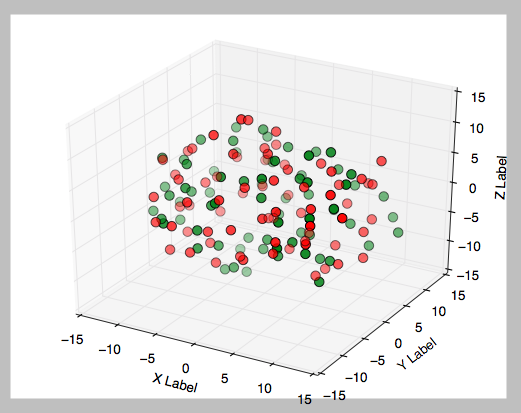
\includegraphics[scale=0.5]{mds}}
where the red points indicate original position and green ones as MDS's.
\end{homeworkProblem}

%----------------------------------------------------------------------------------------
%	PROBLEM 3
%----------------------------------------------------------------------------------------

% To have just one problem per page, simply put a \clearpage after each problem

\begin{homeworkProblem}
To calculate RMSD, according to its equation
$$ RMSD(v,w)= \sqrt{\frac{1}{n} \sum_{i=1}^{n}{((v_{ix}-w_{ix})^2+ (v_{iy} - w_{iy})^2+ (v_{iz}-w_{iz})^2)}} $$
In code,
\begin{lstlisting}
# Calculate RMSD
RMSD = np.sqrt(((X_true - pos)**2).sum() / n_samples)
print RMSD
\end{lstlisting}
The output value of RMSD is $RMSD = 15.876$
\end{homeworkProblem}

%----------------------------------------------------------------------------------------
%	PROBLEM 4
%----------------------------------------------------------------------------------------

% To have just one problem per page, simply put a \clearpage after each problem

\begin{homeworkProblem}
To add noise, the code is as follows.
\begin{lstlisting}
# Add noise to the similarities
noise = np.random.rand(n_samples, n_samples)
noise = noise + noise.T
noise[np.arange(noise.shape[0]), np.arange(noise.shape[0])] = 0
similarities += noise
\end{lstlisting}
After that we follow the same process to apply MDS and calculate RMSD.
The generated graph is as follows. \\
\centerline{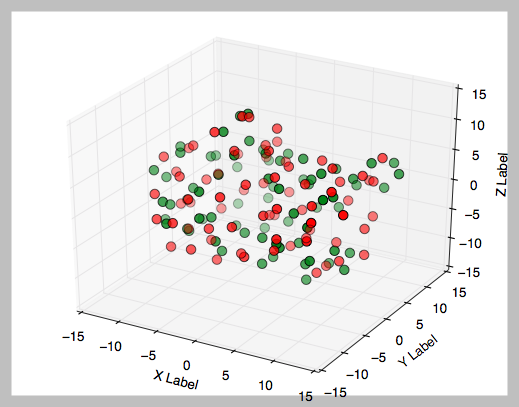
\includegraphics[scale=0.5]{mds2}}
$$ RMSD = 11.6003 $$
(I ran it several times with same seed, the value is always around this value.) The red points indicate original positions of atoms, the green points indicate the generated positions from MDS, given their original difference.
\end{homeworkProblem}

\end{document}